\documentclass[12pt]{report}
\usepackage{parskip}
\usepackage{float}
\floatstyle{boxed}
\restylefloat{figure}
\usepackage{graphicx}
\graphicspath{ {./images/} }
\usepackage{mathptmx}
\usepackage{rotating}
\usepackage{geometry}
\geometry{
a4paper,
total={210mm, 297mm},
left=1.5in,
right=1in,
top=1in,
bottom=1in,
}
\usepackage{fancyhdr}
\fancypagestyle{mystyle}{%
  \fancyhf{}
  \fancyhead[L]{Software Systems Lab}
  \fancyhead[R]{Assignment-1}
  \fancyfoot[L]{IIT Delhi}
  \fancyfoot[R]{\thepage}
  \renewcommand{\headrulewidth}{0.4pt}
  \renewcommand{\footrulewidth}{0.4pt}
}
\pagestyle{mystyle}

\begin{document}

\title{ARMv8 Simulator}
\author{Harshit Patel, Swarnadeep Saha}
\maketitle

\section*{Introduction}
ARMv8 simulator is developed to simulate limited instruction set of ARMv8 architecture in pipelined fashion. It is equipped with a debugger having a set of very useful functionalities.

\section*{Assumptions}
\begin{enumerate}
\item{There are five stages in processor pipeline, namely Instruction Fetch (IF), Instruction Decode (ID), Execution (EX), Memory Access (MA), Write Back (WB).}
\item{Instruction cache and data cache are saperate functional units.}
\item{All attempts to access data from instruction cache and data cache are hits.}
\item{All memory words are 0s unless something is stored into memory through program.}
\item{Functional unit to shift bits in operands of instruction is implemented as combinational circuit and has 0 latency.}
\item{Total 3 cycles are required to fetch an instruction from instruction cache and \bf{2 extra cycles are not considered stall cycles}.}
\item{There are two separate register files:}
\begin{enumerate}
\item{Interger Register File (intRF) of 32 64-bit registers.}
\item{Float Register File (floatRF) of 32 128-bit registers.}
\end{enumerate}
\item{Operands can be forwarded from EX/MA interstage register and MA/WB interstage register in operand forwarding mode.}
\item{Switching happens every cycle in a functional unit for the duration it is active.}
\end{enumerate}

\section*{Source Files}
All source files are in [project\_path]/ARMv8/ folder. Majority of source files have names of the format [stage\_function]\_[instruction\_class].py where [stage\_function] and [instruction\_class] are as below:
\begin{itemize}
\item{[stage\_function]:}
\begin{itemize}
\item{\textbf{opfetch}: These files contain code for decoding and operand fetching for instructions of [instruction\_class] in ID stage.}
\item{\textbf{executor}: These files contain code for executing instructions of [instruction\_class] in EX stage.}
\item{\textbf{memaccess}: These files contain code for memory read/write operations for instructions of [instruction\_class] in MA stage.}
\item{\textbf{writeback}: These files contain code for writing results in destination registers for instructions of [instruction\_class] in WB stage.}
\end{itemize}
\item{[instruction\_class]:}
\begin{itemize}
\item{\textbf{ALU}: Implements CLS and CLZ instructions.}
\item{\textbf{FP\_addSub}: Implements scalar and vector varients of FADD and FSUB instructions.}
\item{\textbf{FP\_maxMin}: Implements scalar and vector varients of FMAX and FMIN instructions.}
\item{\textbf{adc}: Implements ADC instruction.}
\item{\textbf{addSub}: Implements ADD, ADDS, SUB and SUBS instructions.}
\item{\textbf{bitwise\_shift}: Implements  instructions.}
\item{\textbf{branch}: Implements B, BCOND, BL, BR, BLR, RET, CBZ and CBNZ instructions.}
\item{\textbf{conditional}: Implements CSET, CSINC, CNEG, CSNEG, CSINV and CSINV instructions.}
\item{\textbf{loadStore}: Implements LDR, LDRB, LDRSB, LDRH, LDRSH, LDRSW, LDP, STR and STP instructions.}
\item{\textbf{logical}: Implements AND and ANDS instructions.}
\item{\textbf{misc}: Implements ADR, ADRP and NOP instructions.}
\item{\textbf{mov}: Implements MOV, FMOV and FMOV general instructions.}
\item{\textbf{moveWide}: Implements MOVK, MOVN and MOVZ instructions.}
\item{\textbf{mulDiv}: Implements UMULL, UDIV and SDIV instructions.}
\item{\textbf{rotate}: Implements ROR instruction.}
\item{\textbf{shift}: Implements LSL, LSR and ASR instructions.}
\end{itemize}
\end{itemize}

There are several other source files as follows:
\begin{itemize}
\item{\textbf{armdebug.py}: Implements debugger.}
\item{\textbf{utilfunc.py}: Implements utility functions for setting/getting registers from register file, storing/loading memory locations, integer and floating point addition/subtraction etc.}
\item{\textbf{const.py}: Implements global constants and flags used for synchronization and decision making.}
\item{\textbf{config.xml}: Contains hardware specifications of processor.}
\item{\textbf{config.py}: Parses config.xml to read hardware specifications of processor into simulator. }
\end{itemize}

\section*{Limitations of Assignment}
\begin{enumerate}
\item{SIMD instructions are unimplemented.}
\item{Actual number of pipeline stages in ARM processor are more than five.}
\item{Instructions reordering and similar techniques are not used to reduce number of stalls.}
\end{enumerate}

\clearpage
\section*{Testcases}
\begin{figure}[!htb]
\caption{Testcase-1 with output}
\centering
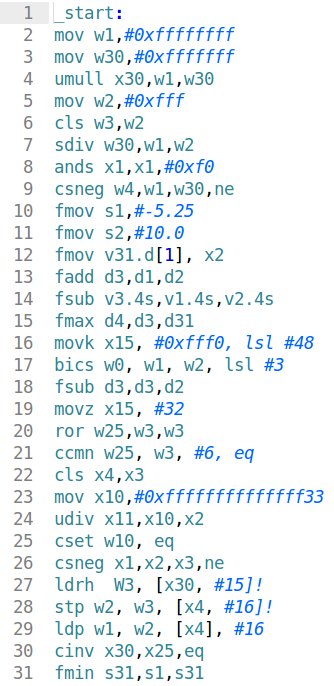
\includegraphics[width=0.30\textwidth]{bench1.png}
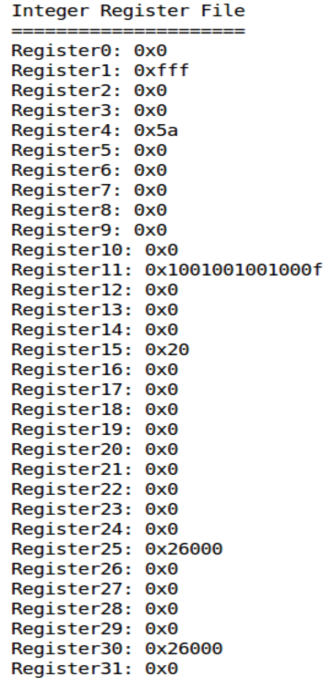
\includegraphics[width=0.30\textwidth]{bench1_intRF.png}
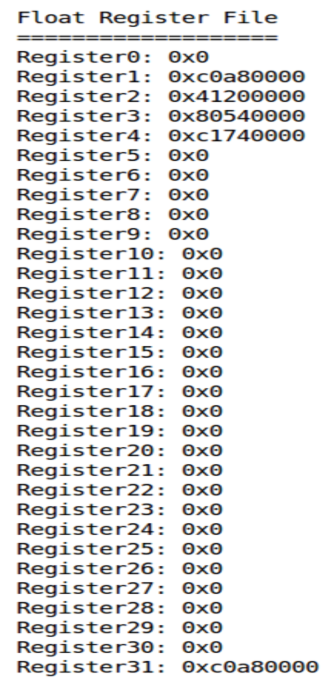
\includegraphics[width=0.30\textwidth]{bench1_floatRF.png}
\end{figure}

\begin{figure}[!htb]
\caption{Testcase-2 with output}
\centering
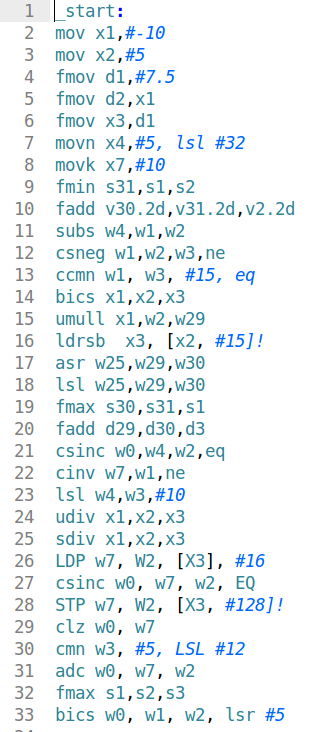
\includegraphics[width=0.30\textwidth]{bench2.png}
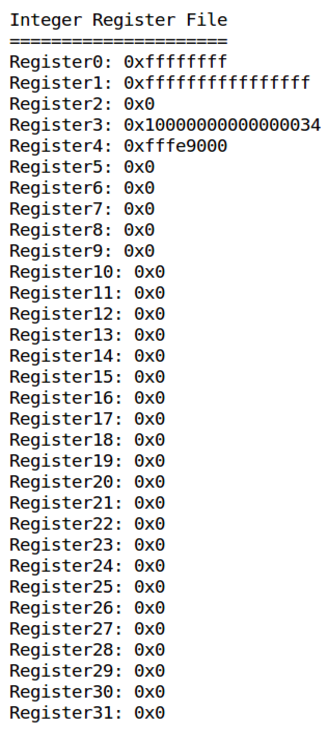
\includegraphics[width=0.30\textwidth]{bench2_intRF.png}
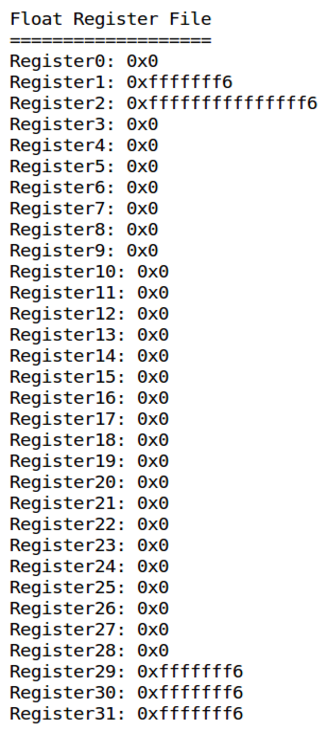
\includegraphics[width=0.30\textwidth]{bench2_floatRF.png}
\end{figure}

\clearpage
\subsection*{Energy vs Voltage Graphs for Testcase-1}
\begin{figure}[!htb]
\begin{sideways}

\caption{Testcase-1 Energy vs Voltage graphs}
\centering
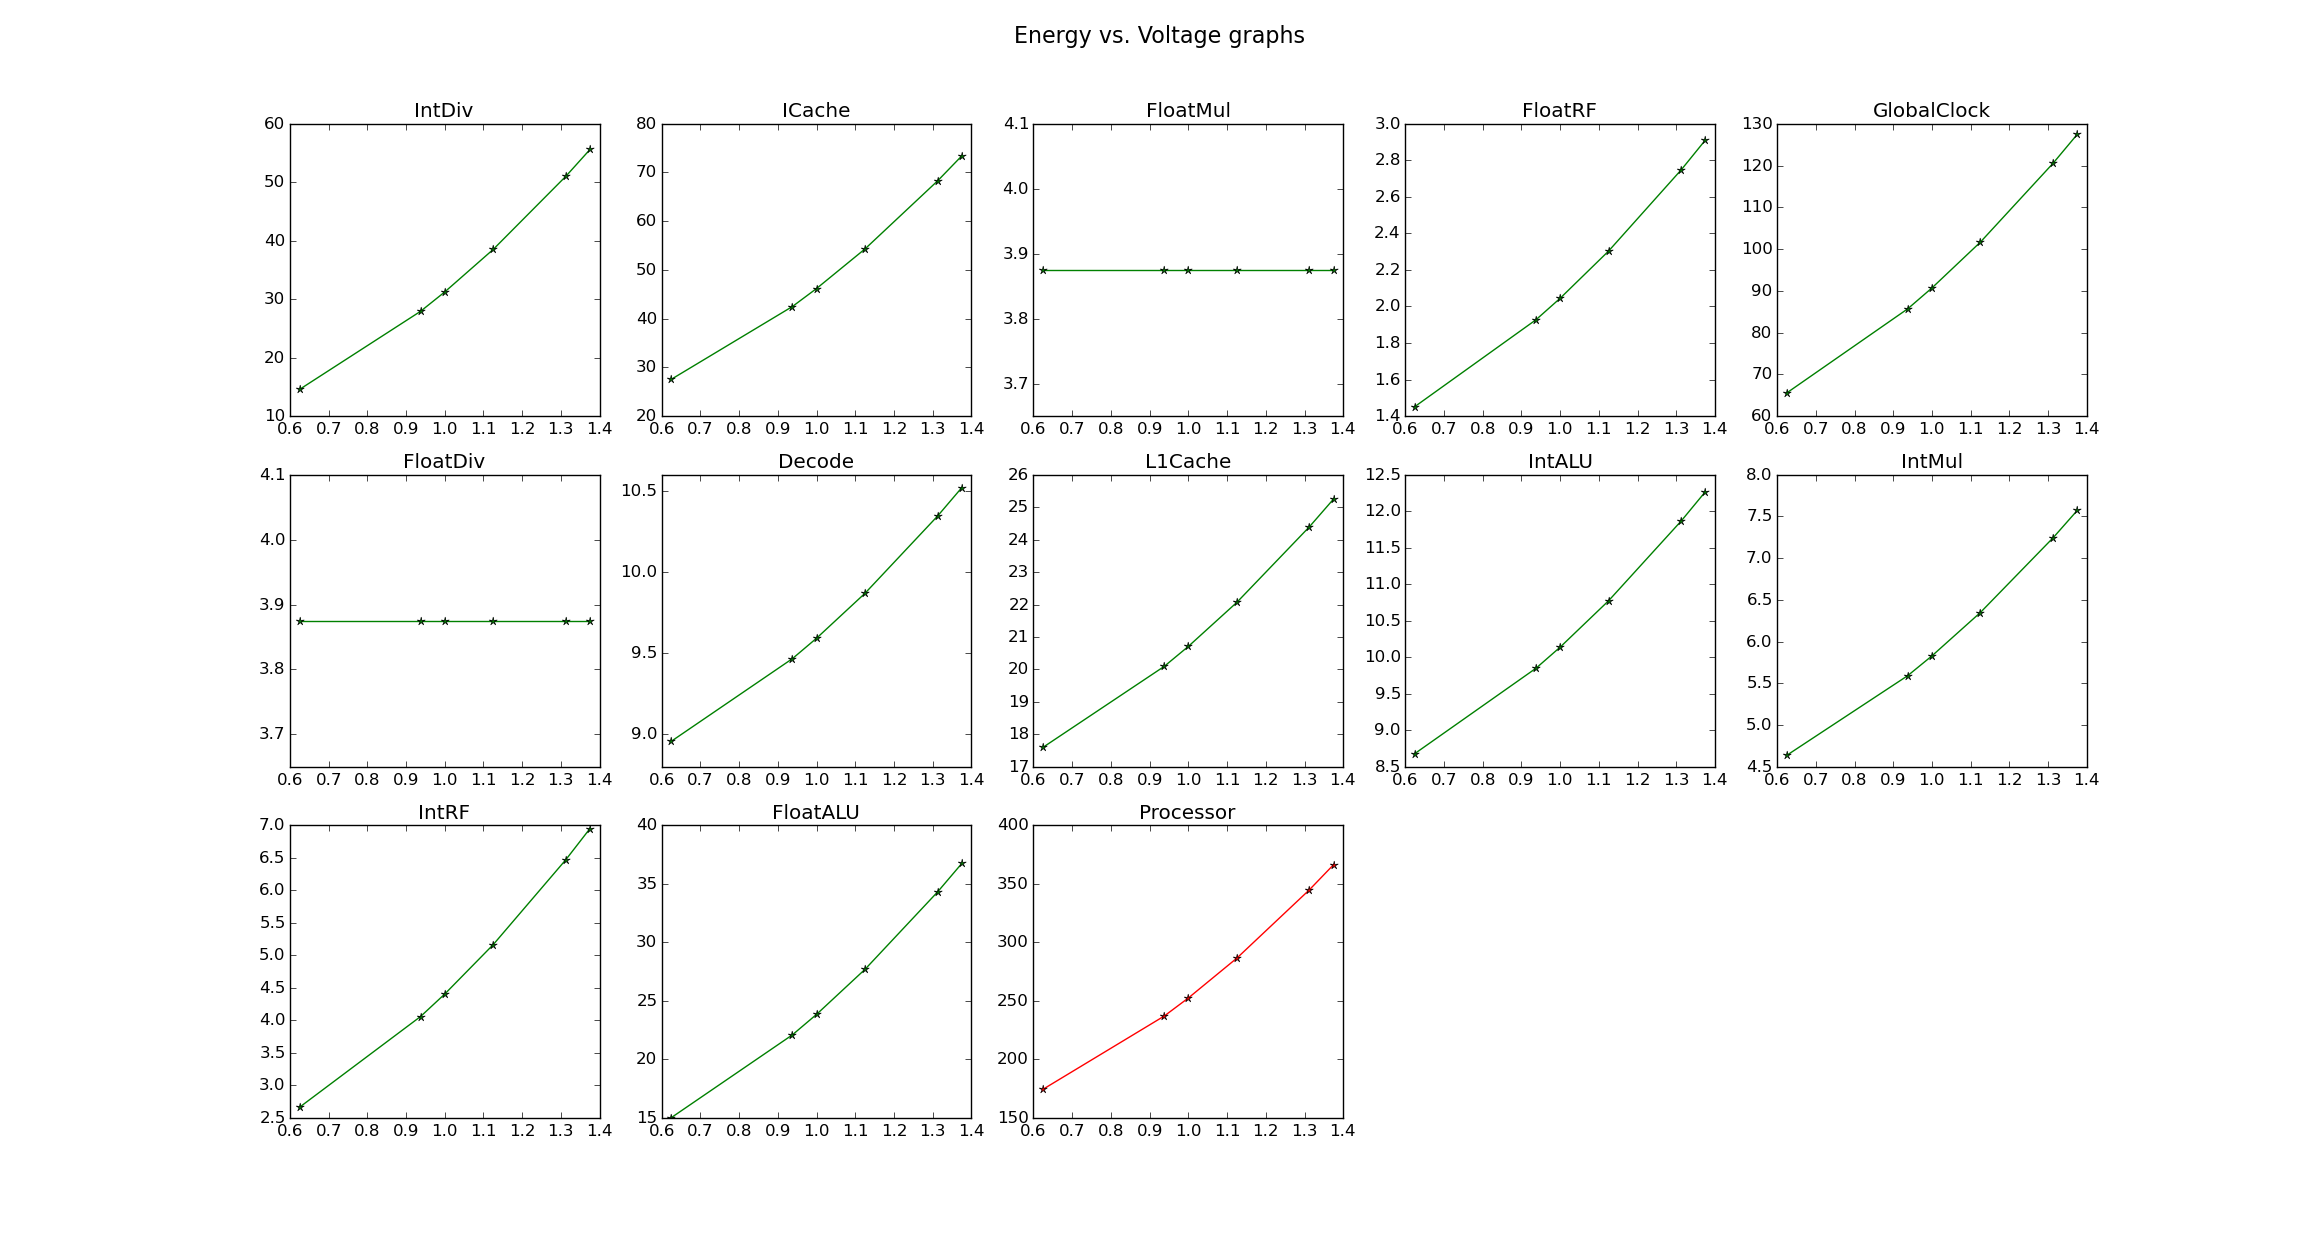
\includegraphics[width=0.9\textheight]{bench1_figure_1.png}

\end{sideways}
\end{figure}

\clearpage
\subsection*{EDP vs Voltage Graphs for Testcase-1}
\begin{figure}[!htb]
\begin{sideways}

\caption{Testcase-1 EDP vs Voltage graphs}
\centering
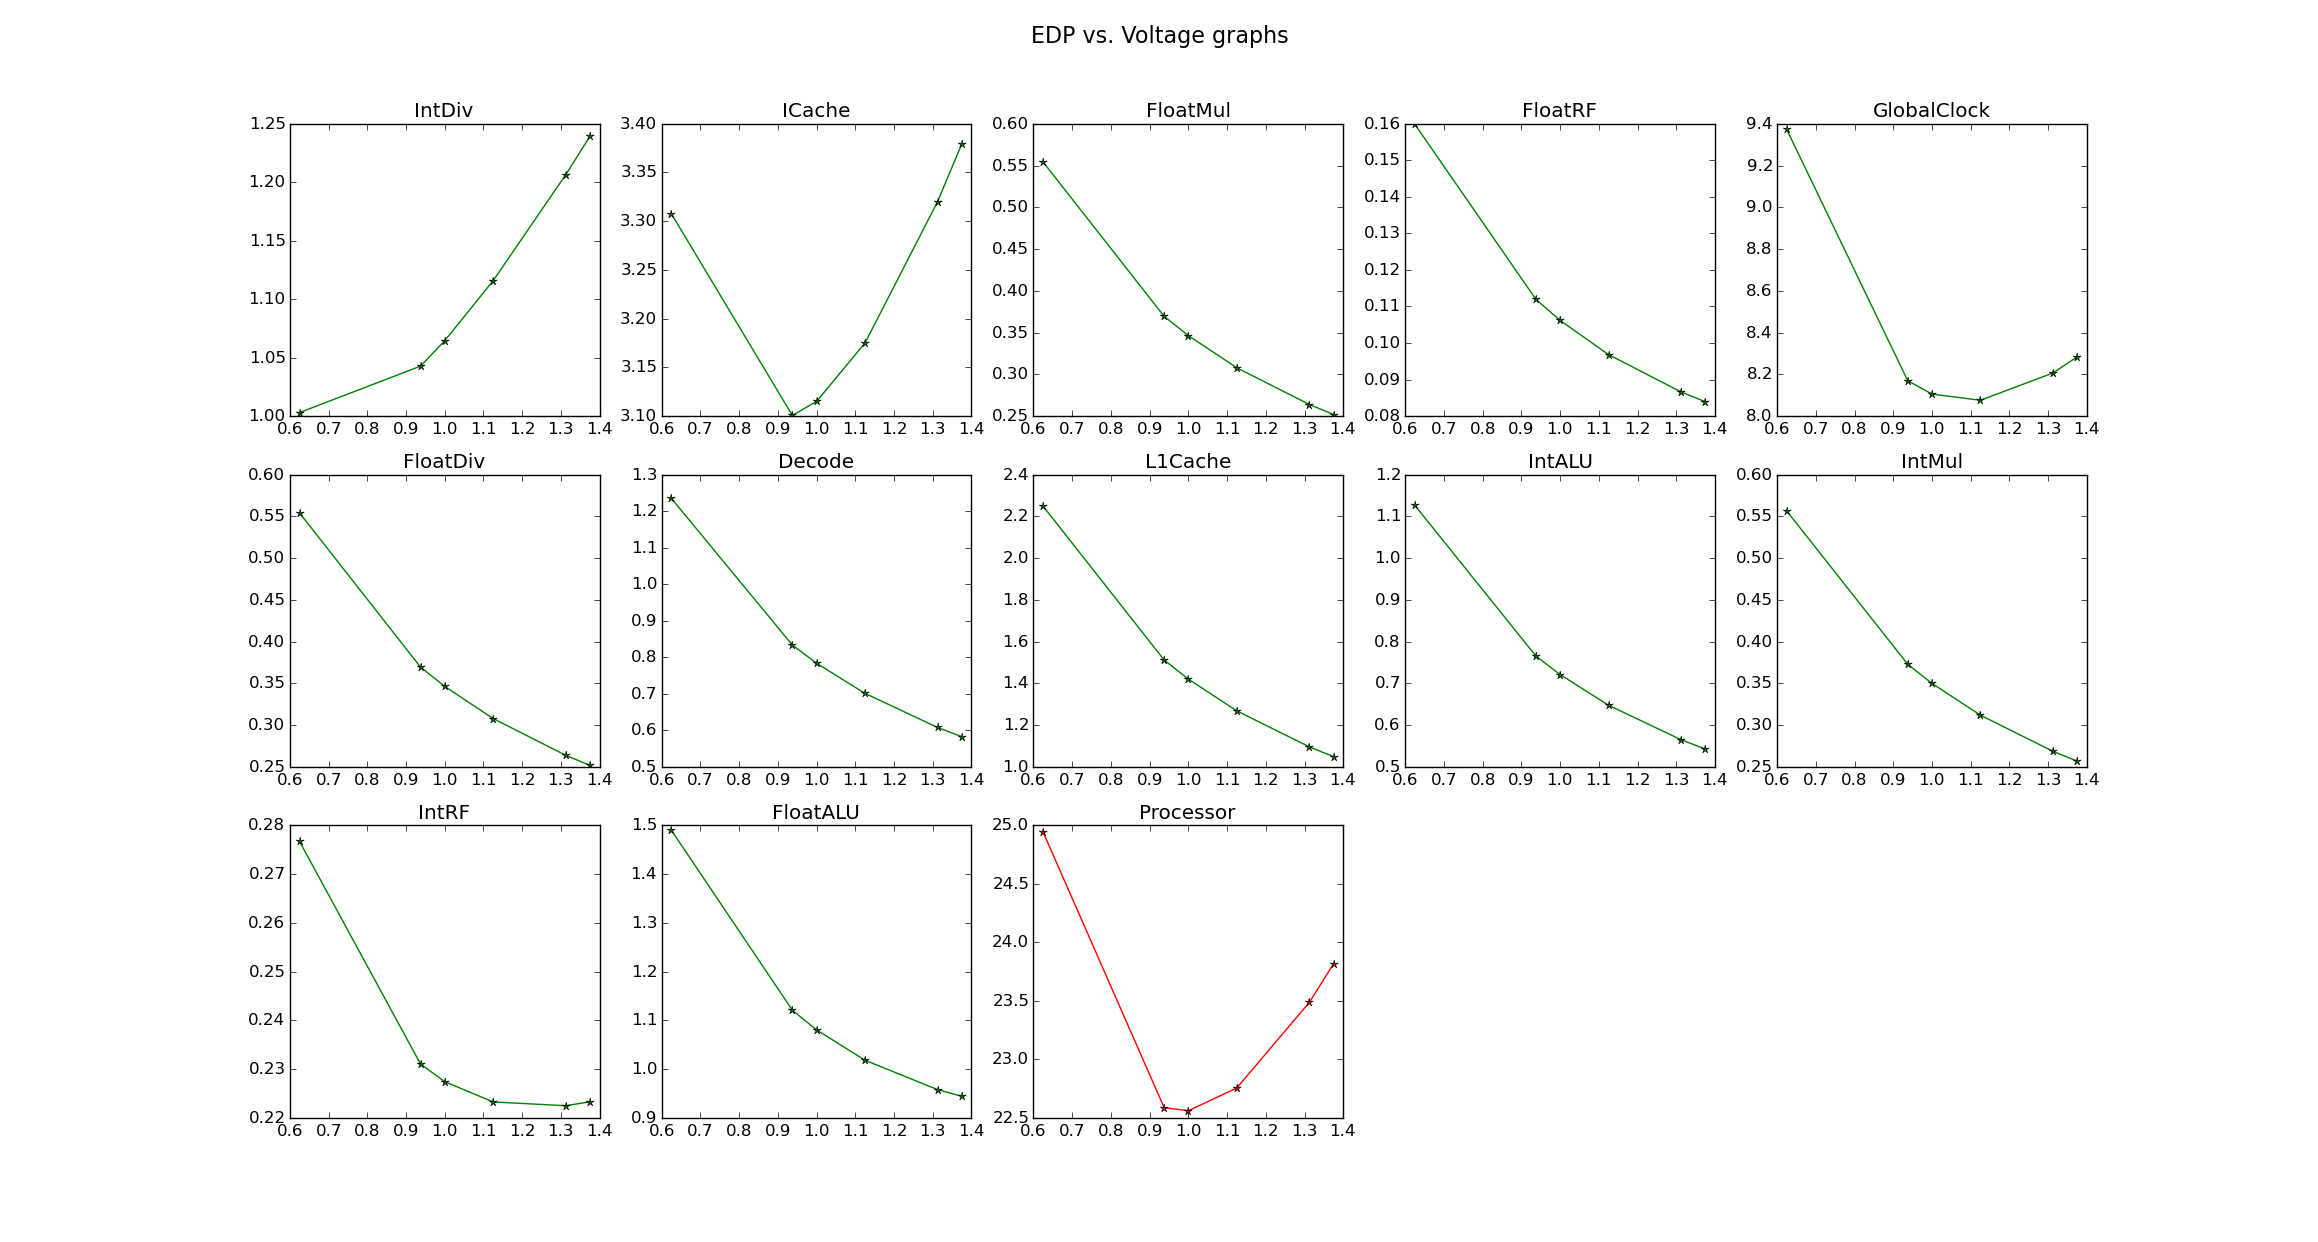
\includegraphics[width=0.9\textheight]{bench1_figure_2.png}

\end{sideways}
\end{figure}

\clearpage
\subsection*{Energy vs Voltage Graphs for Testcase-2}
\begin{figure}[!htb]
\begin{sideways}

\caption{Testcase-2 Energy vs Voltage graphs}
\centering
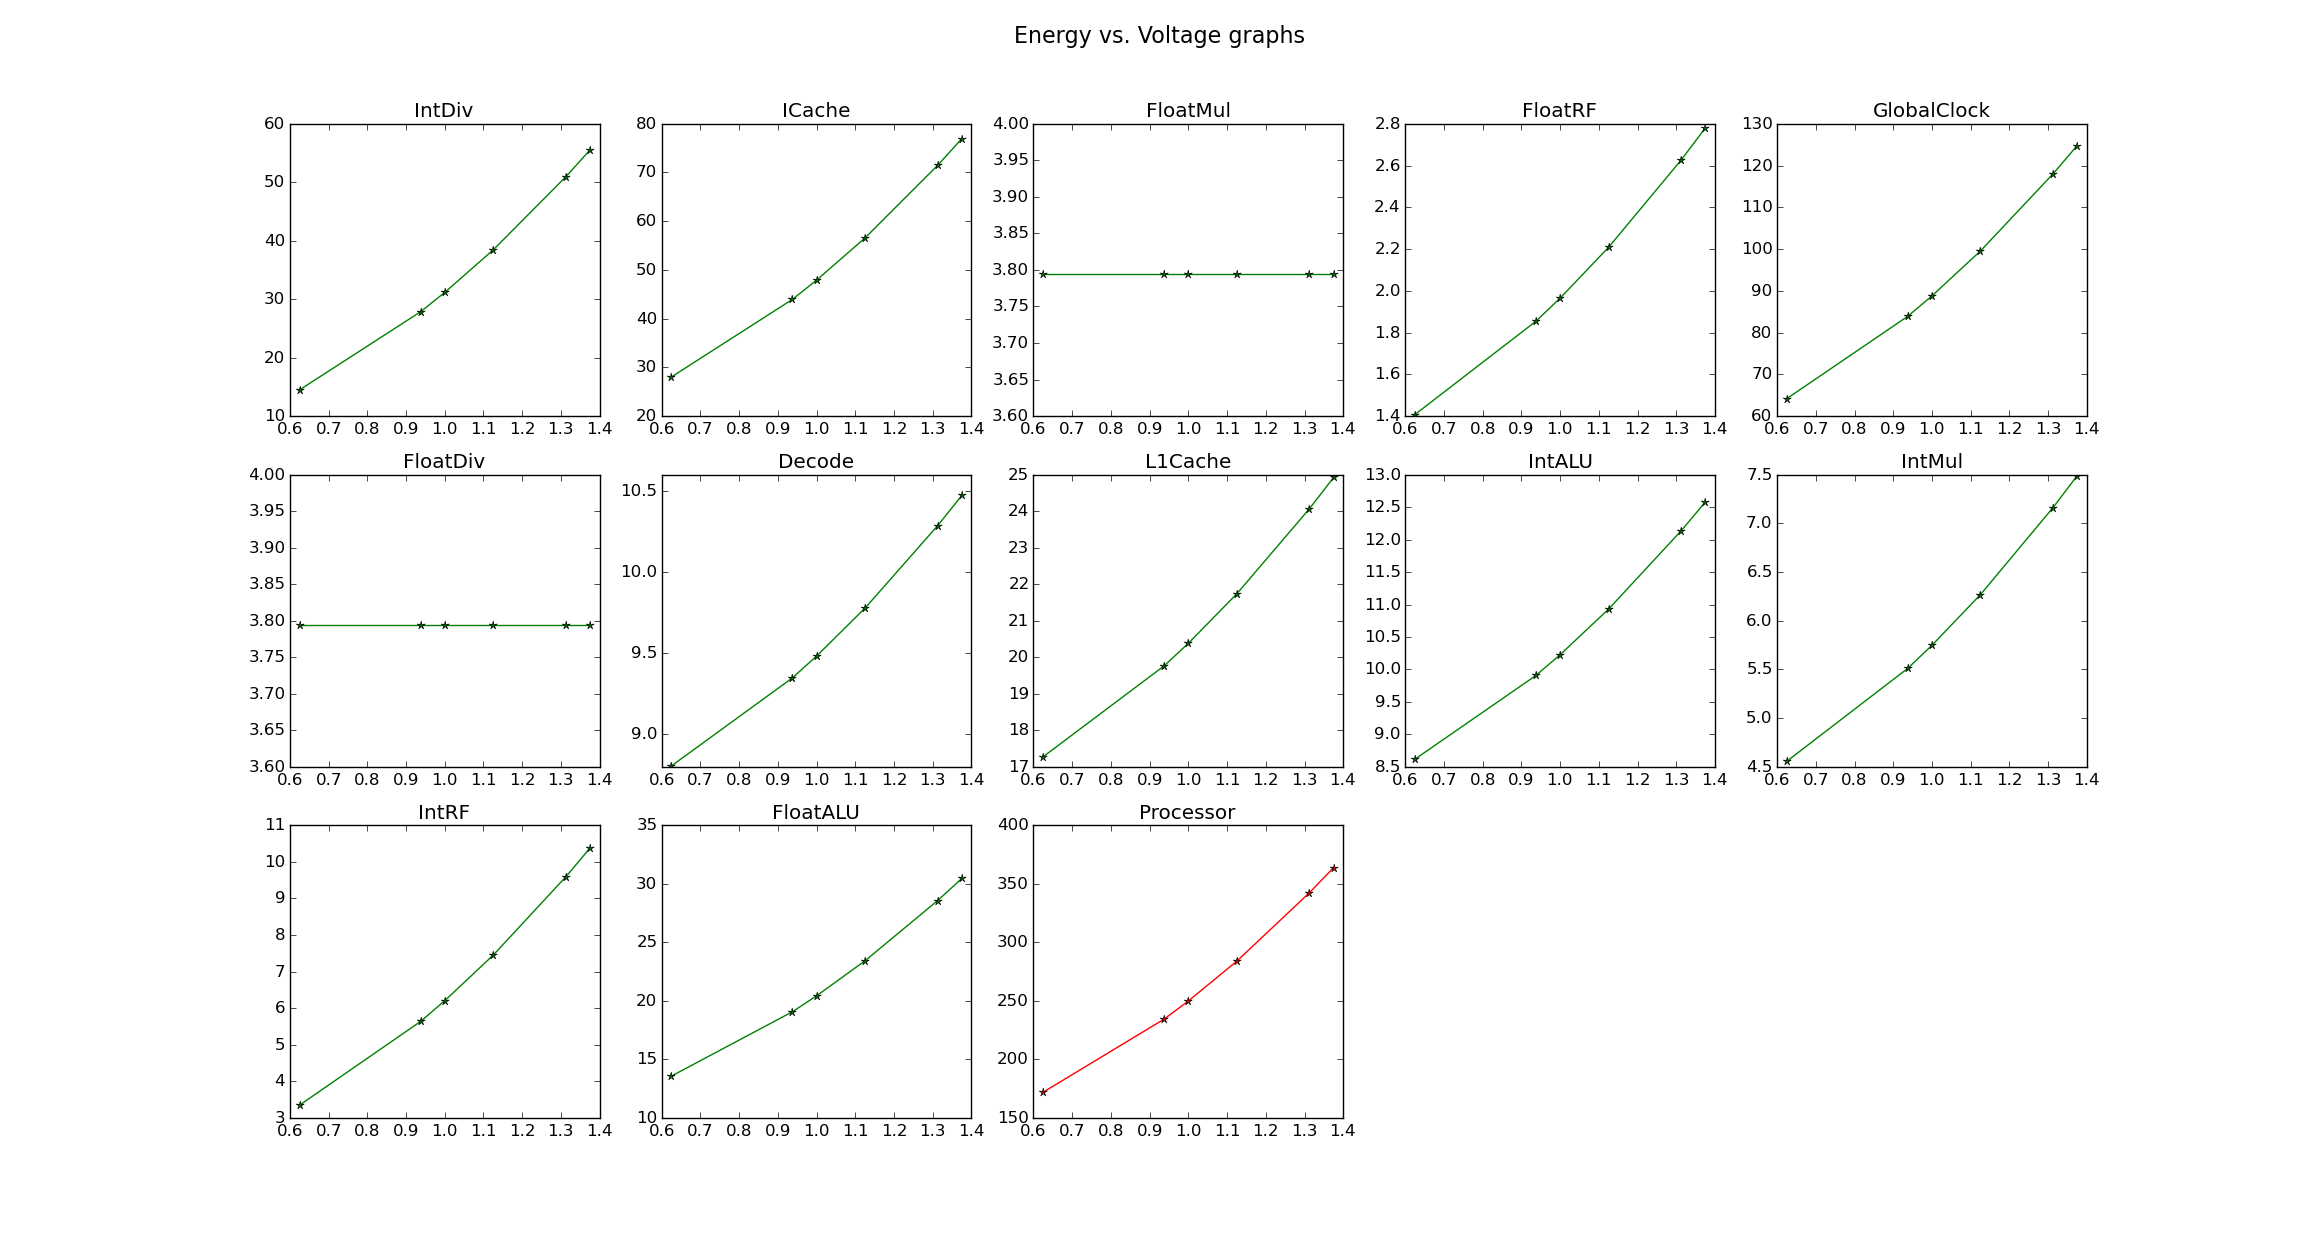
\includegraphics[width=0.9\textheight]{bench2_figure_1.png}

\end{sideways}
\end{figure}

\clearpage
\subsection*{EDP vs Voltage Graphs for Testcase-2}
\begin{figure}[!htb]
\begin{sideways}

\caption{Testcase-2 EDP vs Voltage graphs}
\centering
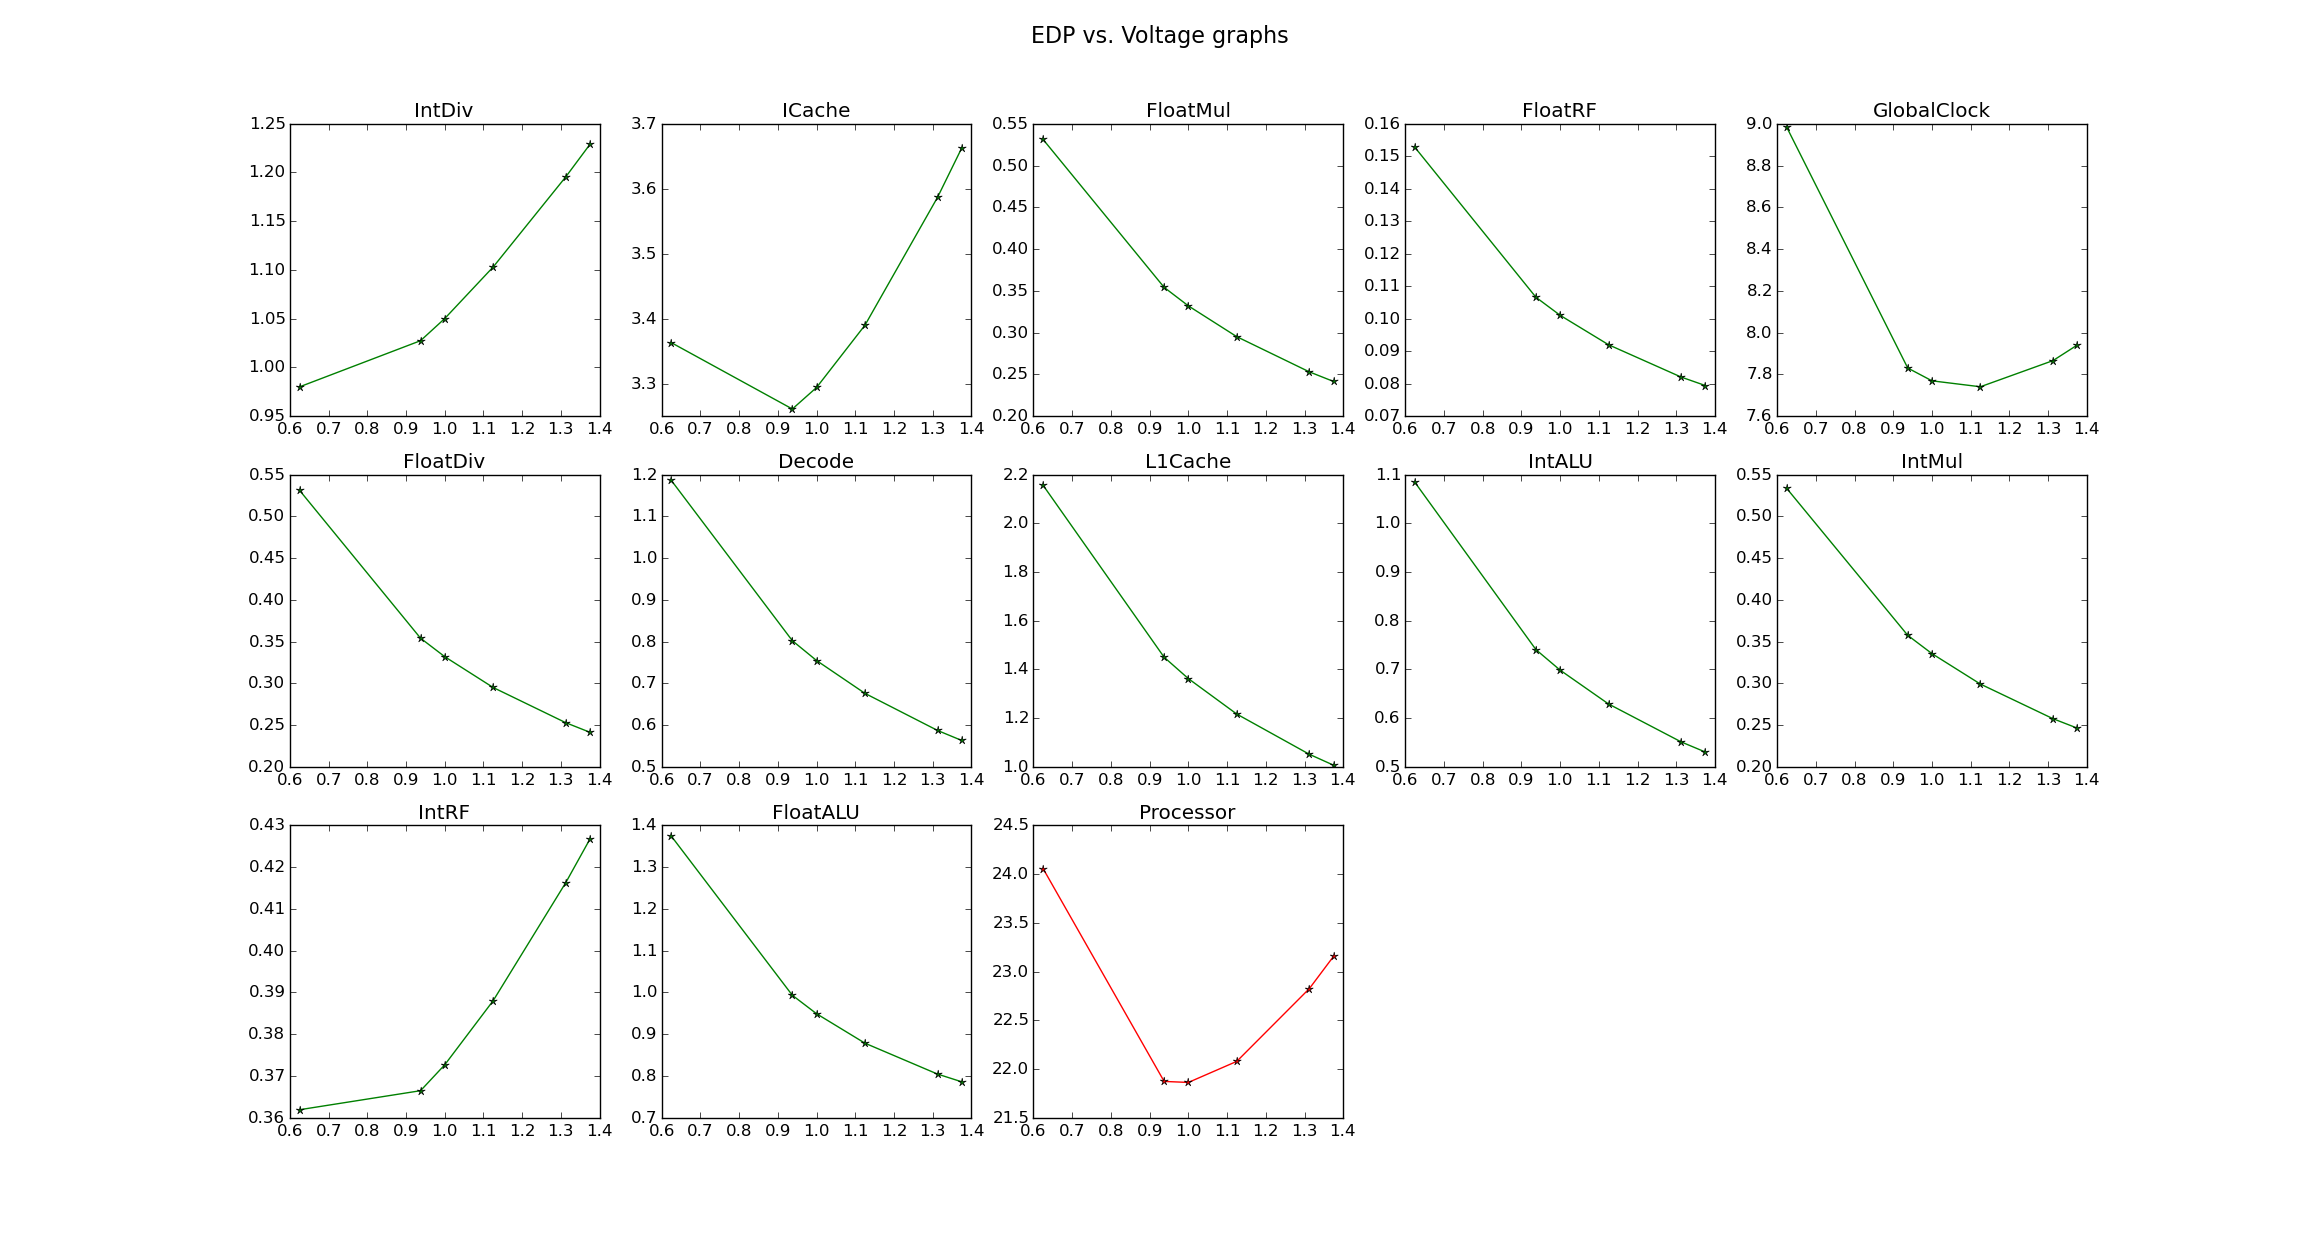
\includegraphics[width=0.9\textheight]{bench2_figure_2.png}

\end{sideways}
\end{figure}



\end{document}